\documentclass[12pt, a4paper]{article}
\usepackage[UTF8, zihao=-4]{ctex}
\usepackage{fontspec}
\setmainfont{Times New Roman}
\usepackage[top=1.5cm, bottom=1.5cm, left=1.2cm, right=1.2cm, headheight=15pt, includehead]{geometry}
\usepackage{graphicx}
\usepackage{float}
\usepackage{fancyhdr}
\usepackage{eso-pic}
\usepackage{tikz}
\usepackage{setspace}

% 水印设置（前景层，覆盖图片）
\AddToShipoutPictureFG{%
  \begin{tikzpicture}[overlay, remember picture]
    \node[
      at=(current page.center),
      opacity=0.12,
      rotate=45,
      font=\sffamily\bfseries\fontsize{48}{48}\selectfont,
      text=gray
    ] {叶哲昊\ \ 24012561};
  \end{tikzpicture}%
}

% 页眉页脚
\pagestyle{fancy}
\fancyhf{}
\renewcommand{\headrulewidth}{0.4pt}
\fancyhead[L]{\zihao{5} 电磁场与电磁波\ \ 3.1 静电场分析及应用}
\fancyhead[R]{\zihao{5} 叶哲昊\ 24012561}
\fancyfoot[C]{\thepage}

\setstretch{1.3}

\begin{document}

% 封面标题
\begin{center}
  {\zihao{2}\heiti 3.1 静电场分析及应用}\\[0.5cm]
  {\zihao{4} 例题与习题解析}\\[0.3cm]
  {\zihao{5} 叶哲昊\quad 24012561}
\end{center}

\vspace{0.5cm}
\hrule
\vspace{0.8cm}

% 例 3.1.3
\section*{例 3.1.3}

\begin{figure}[H]
  \centering
  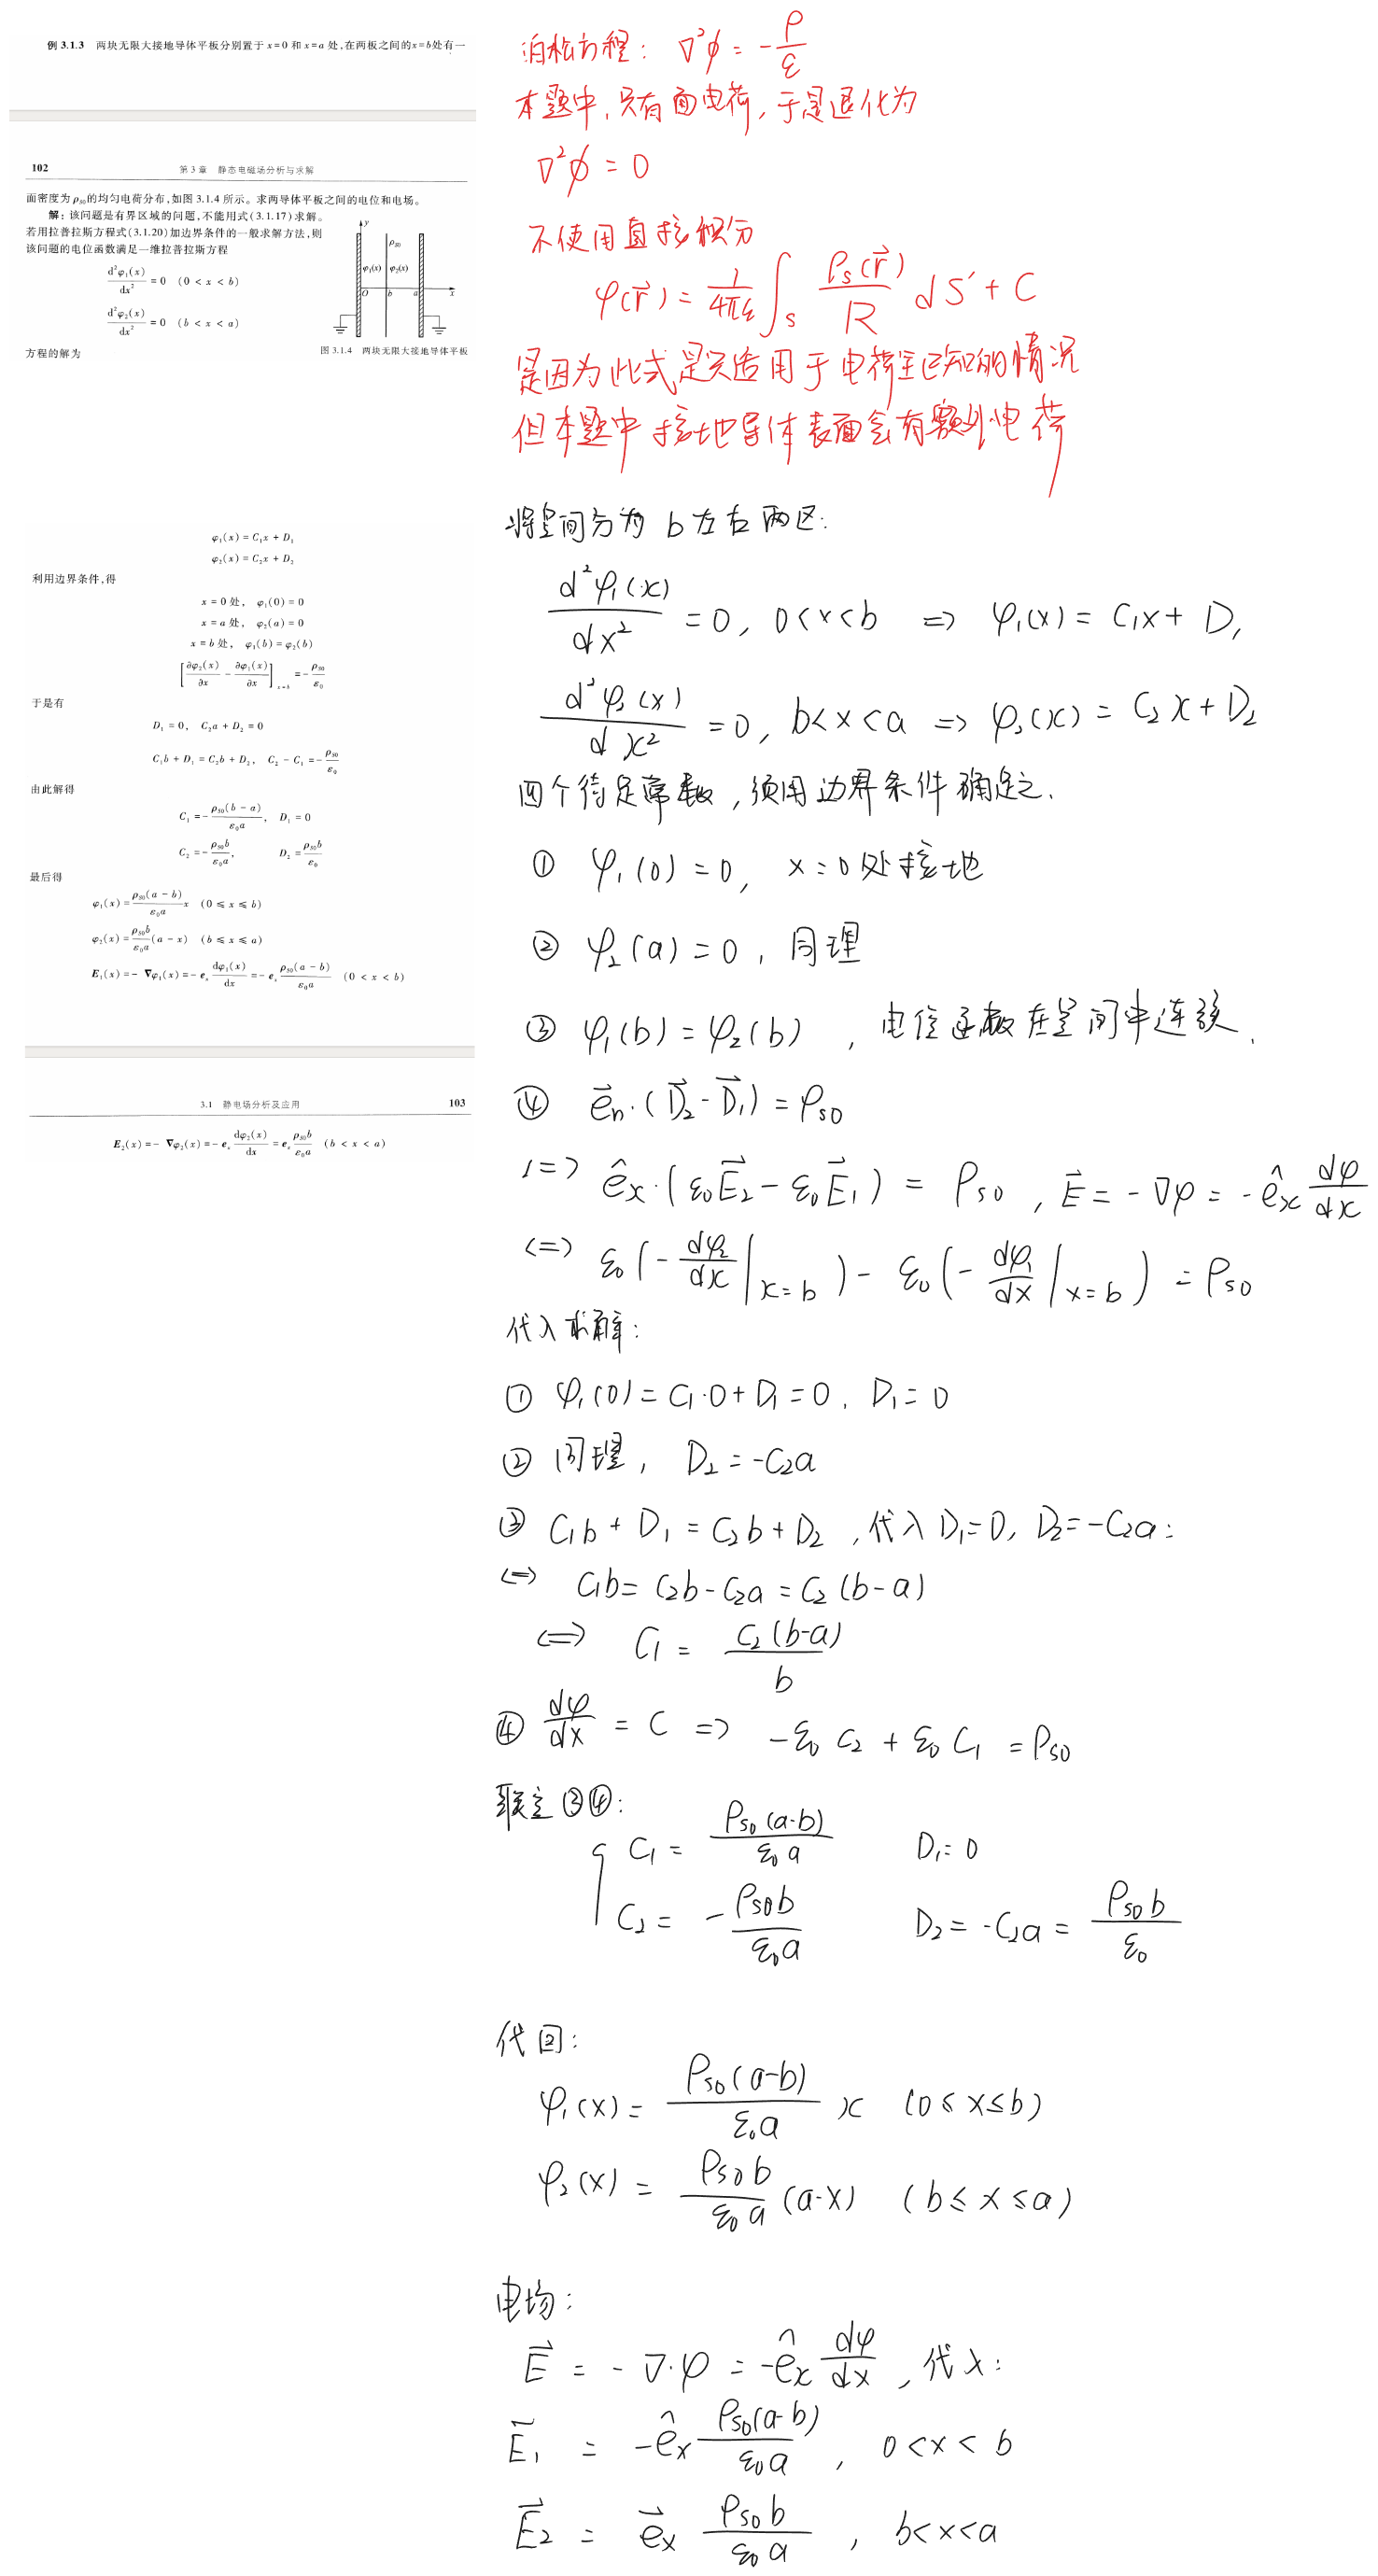
\includegraphics[width=\linewidth, height=0.88\textheight, keepaspectratio]{例 3.1.3.png}
\end{figure}

\clearpage

% 例 3.1.4
\section*{例 3.1.4}

\begin{figure}[H]
  \centering
  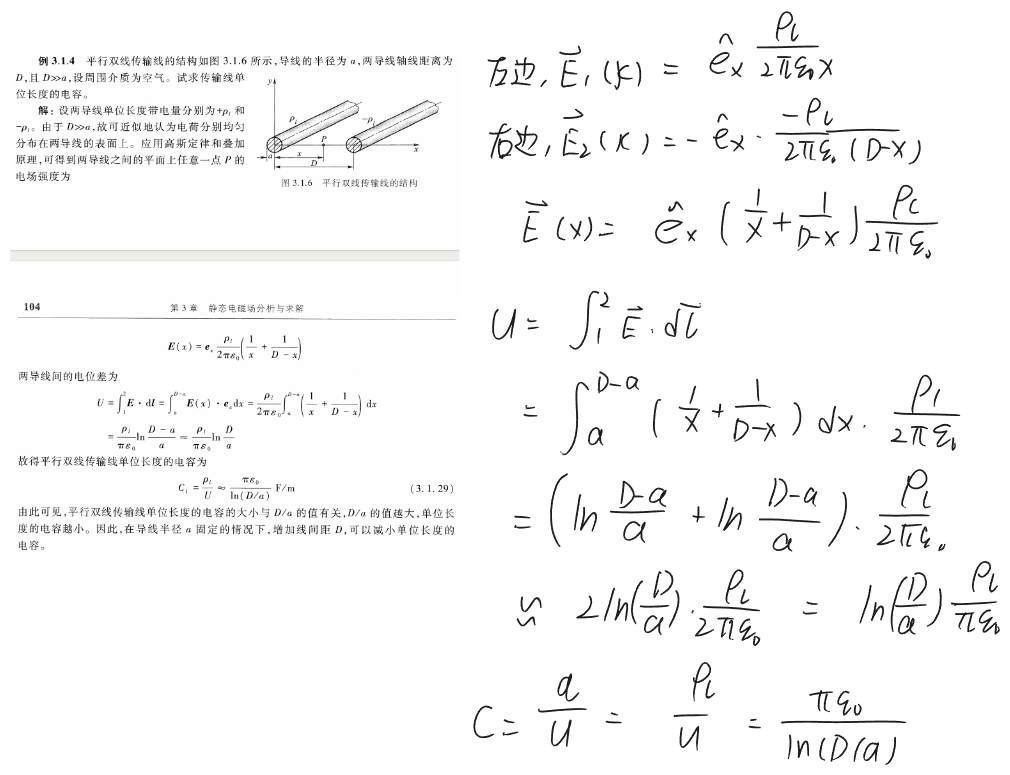
\includegraphics[width=\linewidth, height=0.88\textheight, keepaspectratio]{例 3.1.4.png}
\end{figure}

\clearpage

% 例 3.1.7
\section*{例 3.1.7}

\begin{figure}[H]
  \centering
  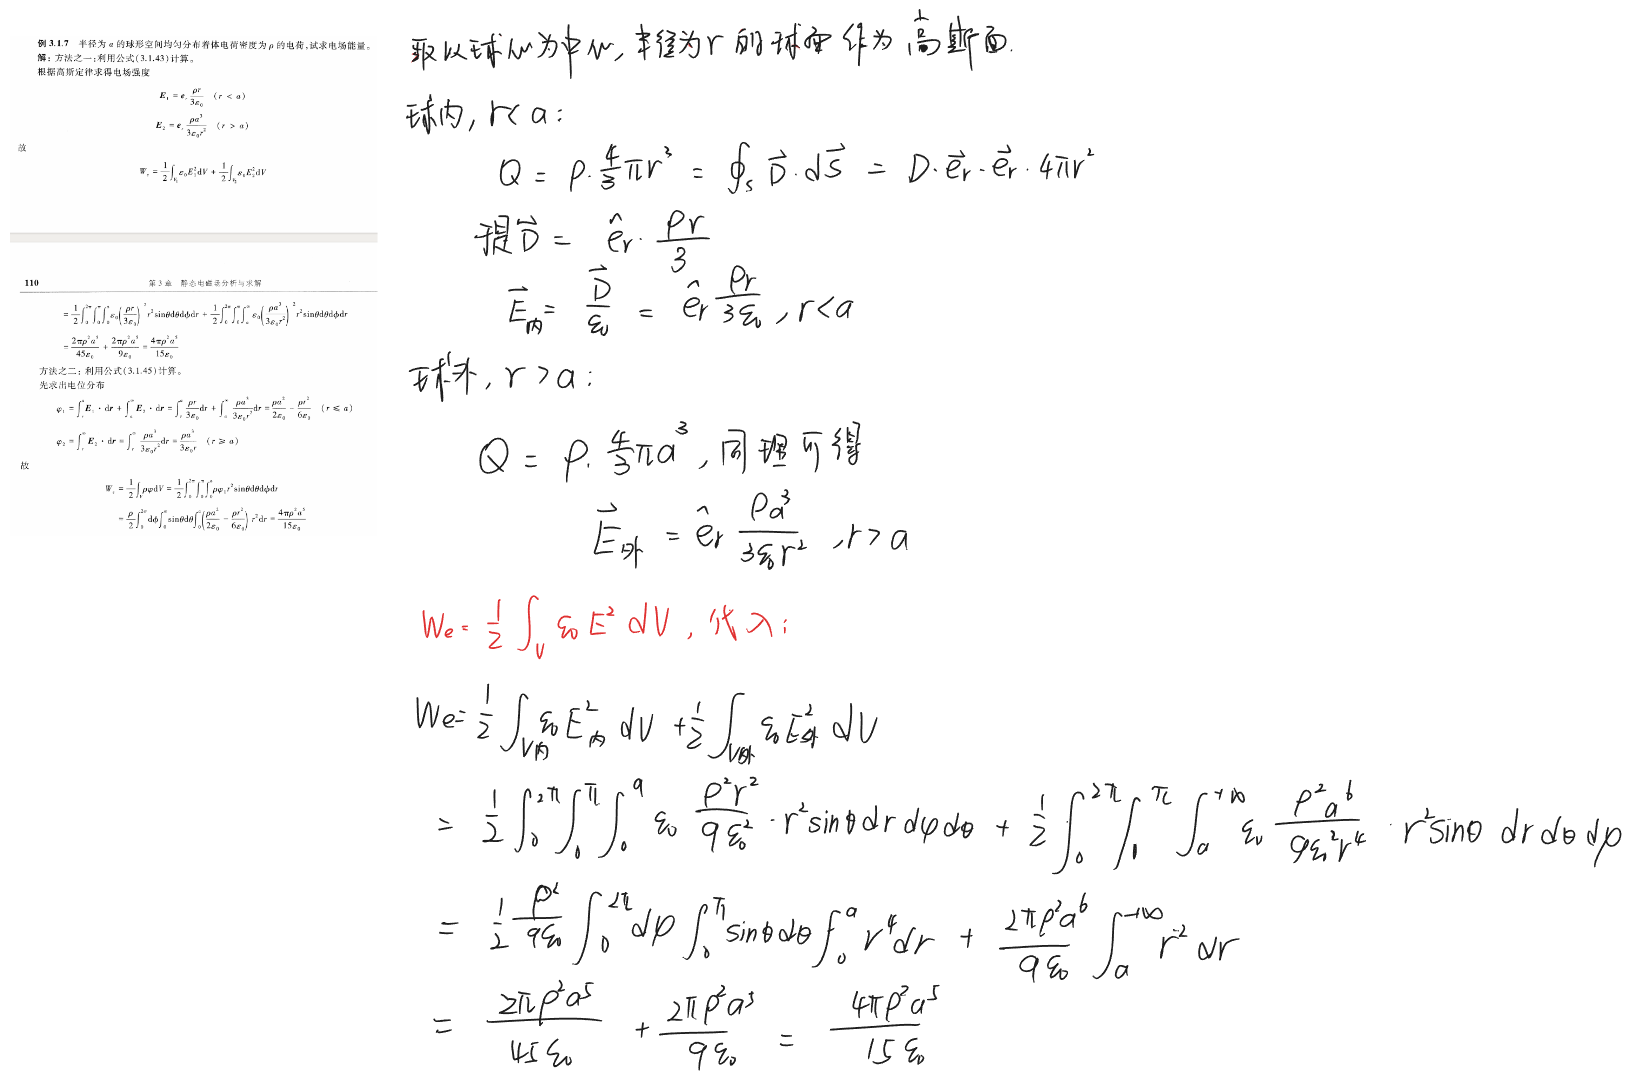
\includegraphics[width=\linewidth, height=0.88\textheight, keepaspectratio]{例 3.1.7.png}
\end{figure}

\clearpage

% 例 3.1.8
\section*{例 3.1.8}

\begin{figure}[H]
  \centering
  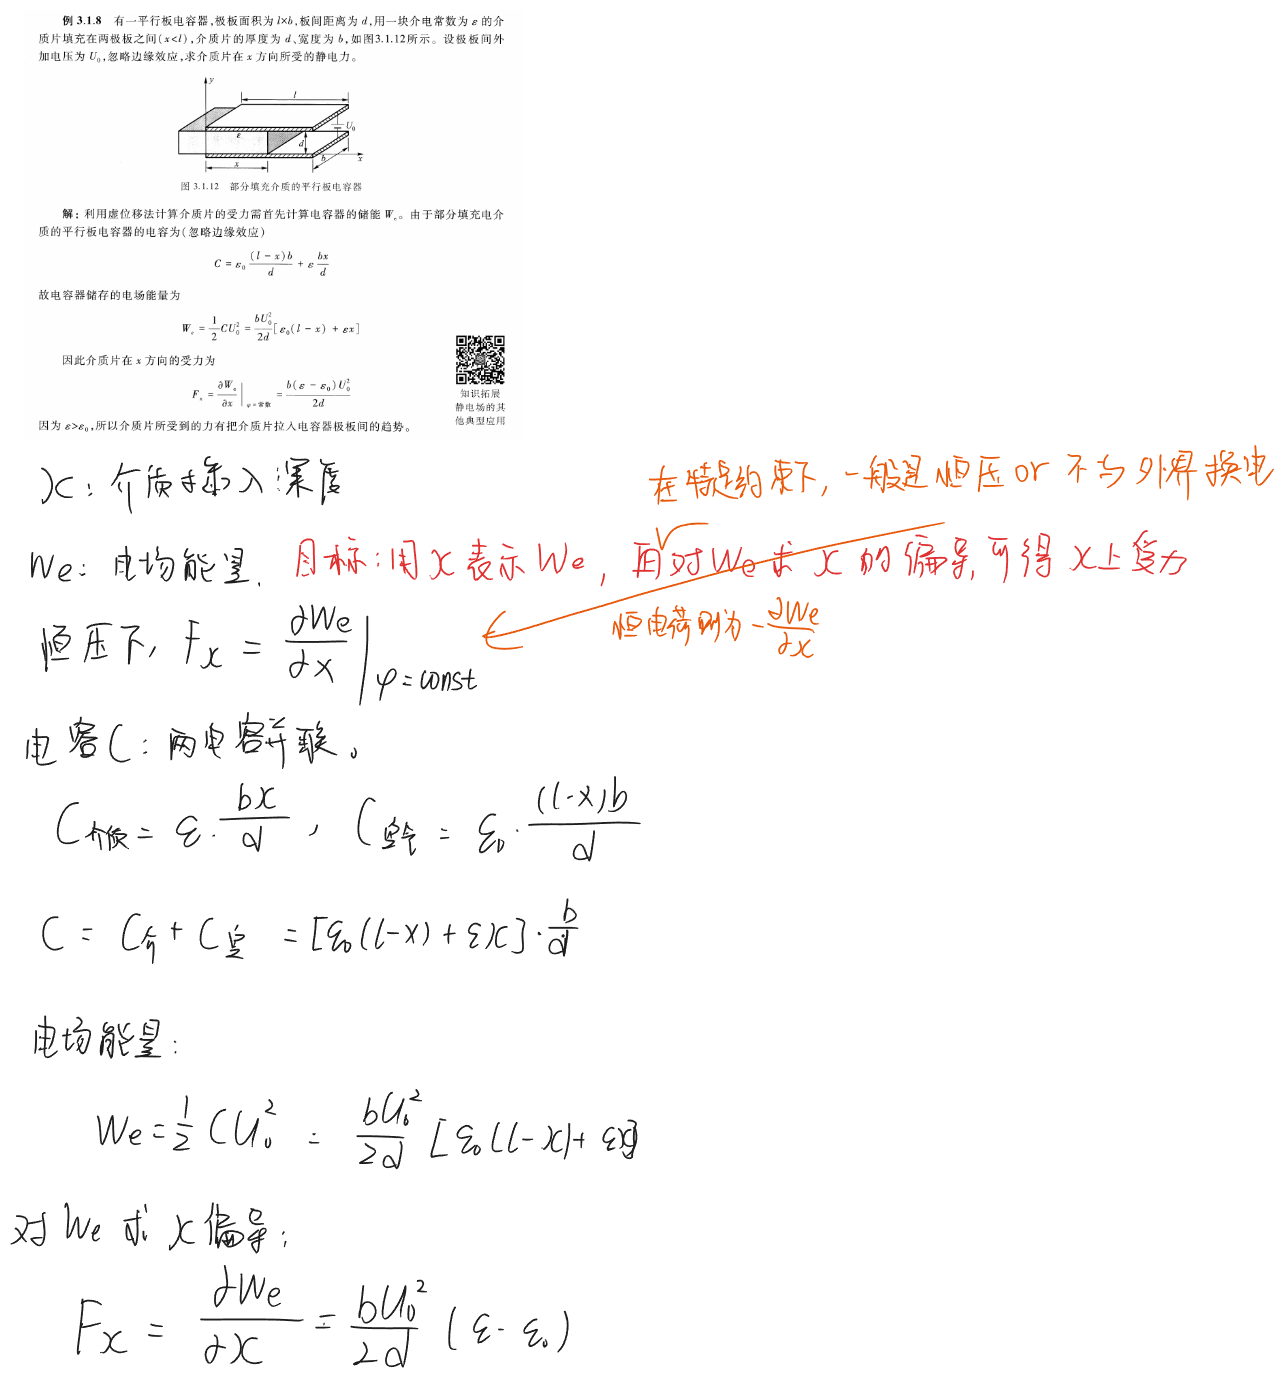
\includegraphics[width=\linewidth, height=0.88\textheight, keepaspectratio]{例 3.1.8.png}
\end{figure}

\clearpage

% 习题 3.1.2
\section*{习题 3.1.2}

\begin{figure}[H]
  \centering
  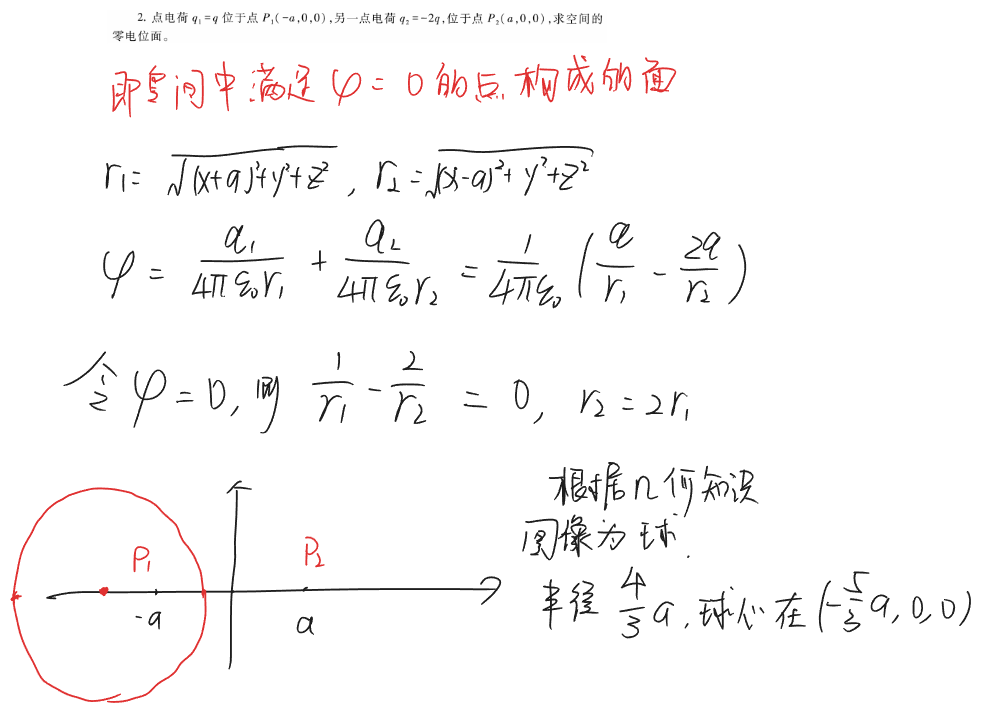
\includegraphics[width=\linewidth, height=0.88\textheight, keepaspectratio]{习题 3.1.2.png}
\end{figure}

\clearpage

% 习题 3.1.3
\section*{习题 3.1.3}

\begin{figure}[H]
  \centering
  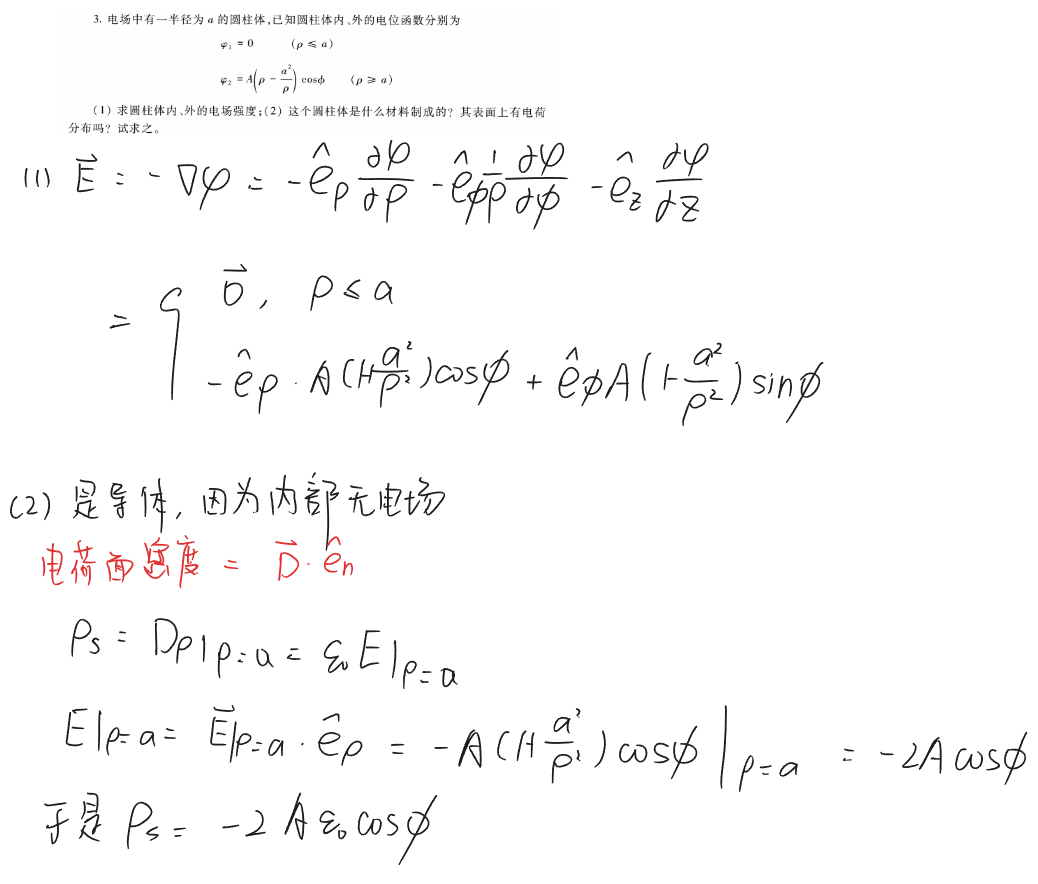
\includegraphics[width=\linewidth, height=0.88\textheight, keepaspectratio]{习题 3.1.3.png}
\end{figure}

\clearpage

% 习题 3.1.5
\section*{习题 3.1.5}

\begin{figure}[H]
  \centering
  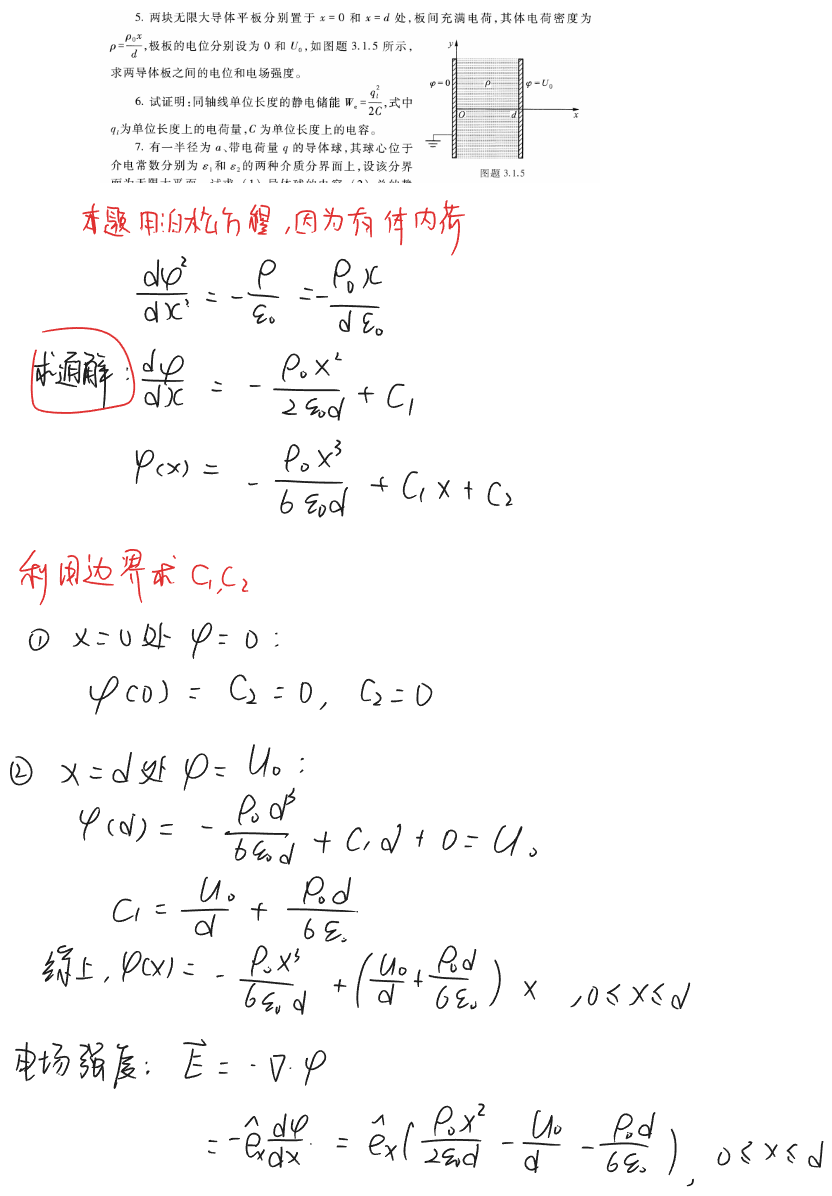
\includegraphics[width=\linewidth, height=0.88\textheight, keepaspectratio]{习题 3.1.5.png}
\end{figure}

\clearpage

% 习题 3.1.6
\section*{习题 3.1.6}

\begin{figure}[H]
  \centering
  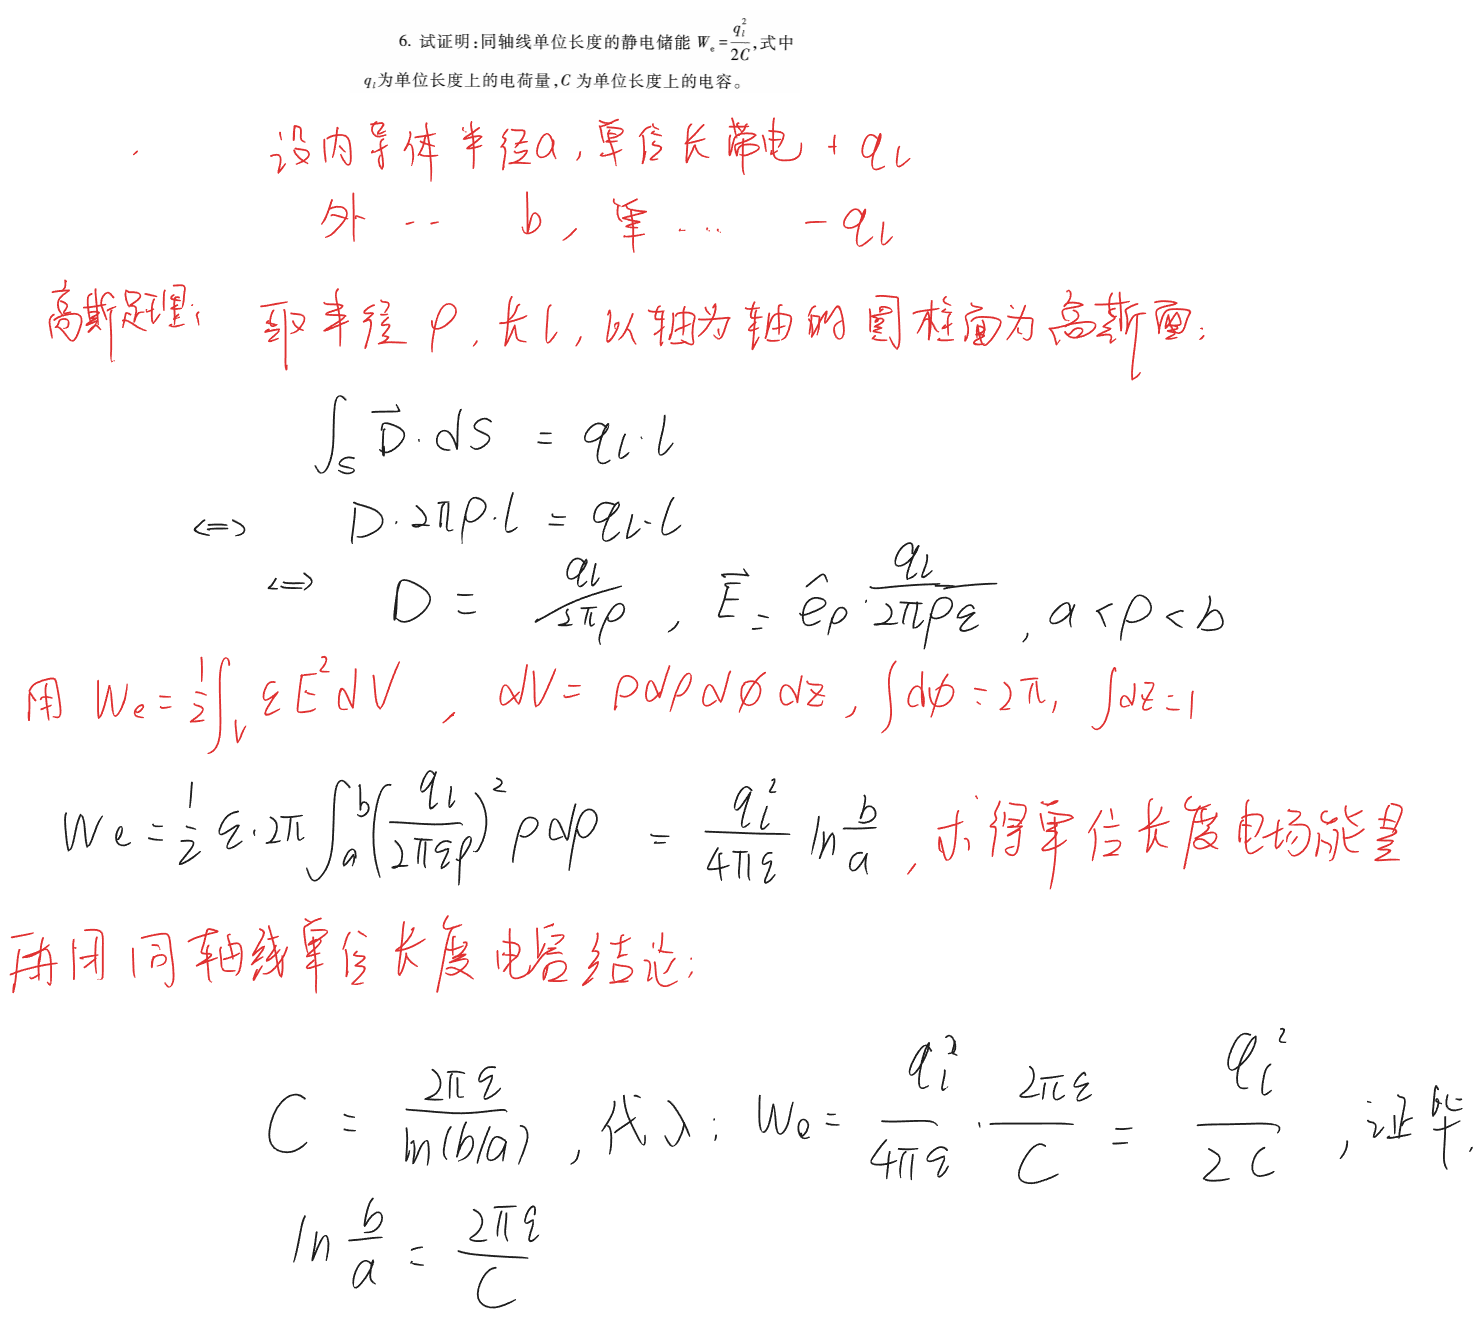
\includegraphics[width=\linewidth, height=0.88\textheight, keepaspectratio]{习题 3.1.6.png}
\end{figure}

\clearpage

% 习题 3.1.7
\section*{习题 3.1.7}

\begin{figure}[H]
  \centering
  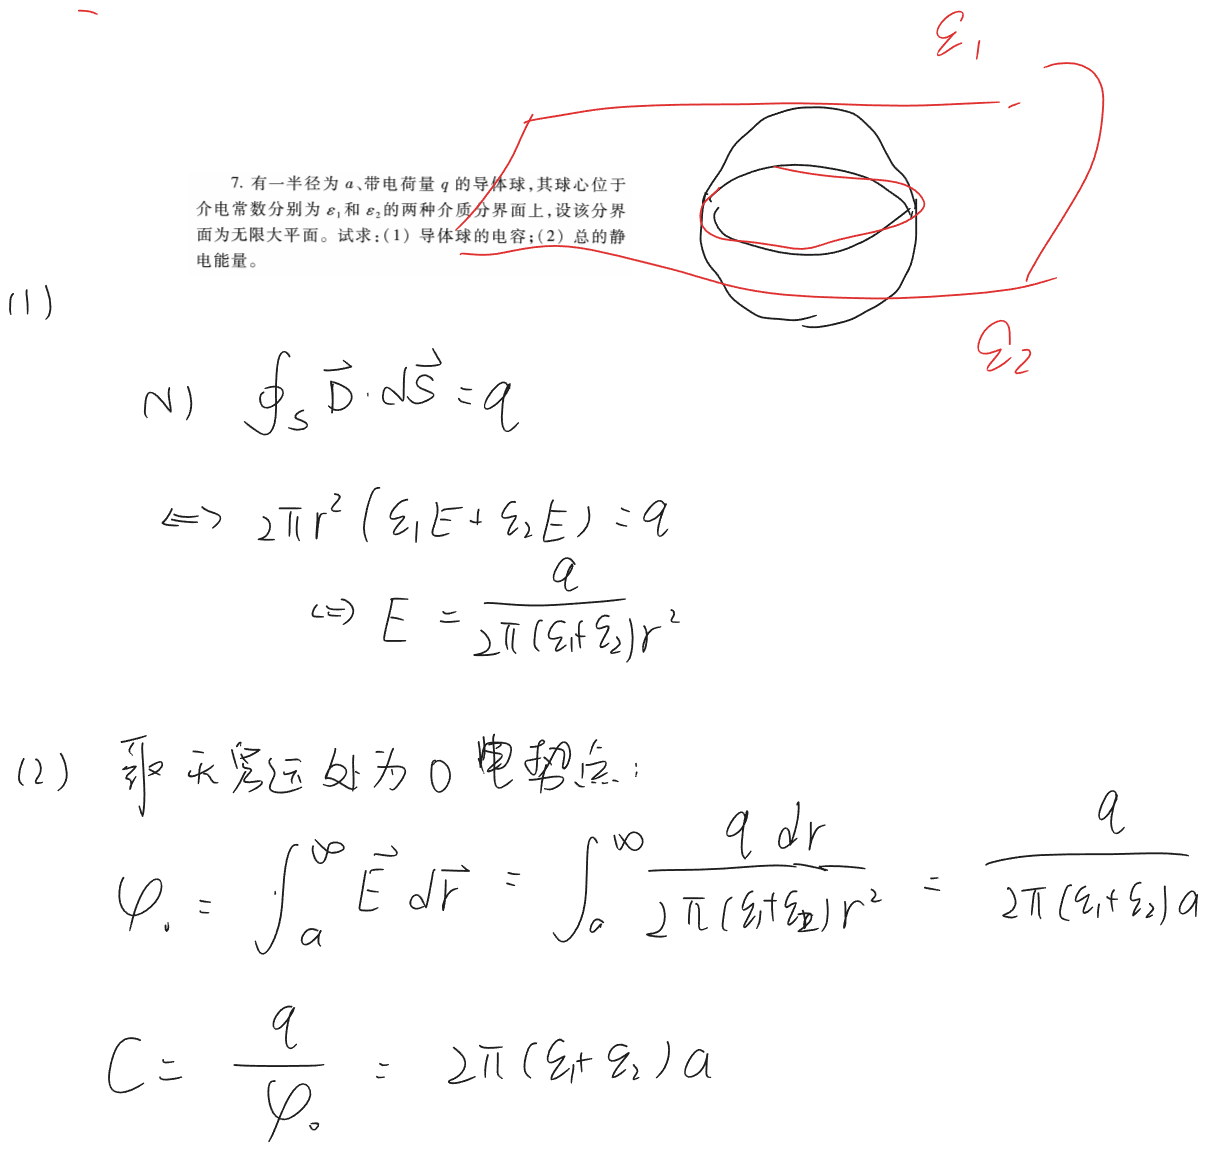
\includegraphics[width=\linewidth, height=0.88\textheight, keepaspectratio]{习题 3.1.7.png}
\end{figure}

\clearpage

% 习题 3.1.11
\section*{习题 3.1.11}

\begin{figure}[H]
  \centering
  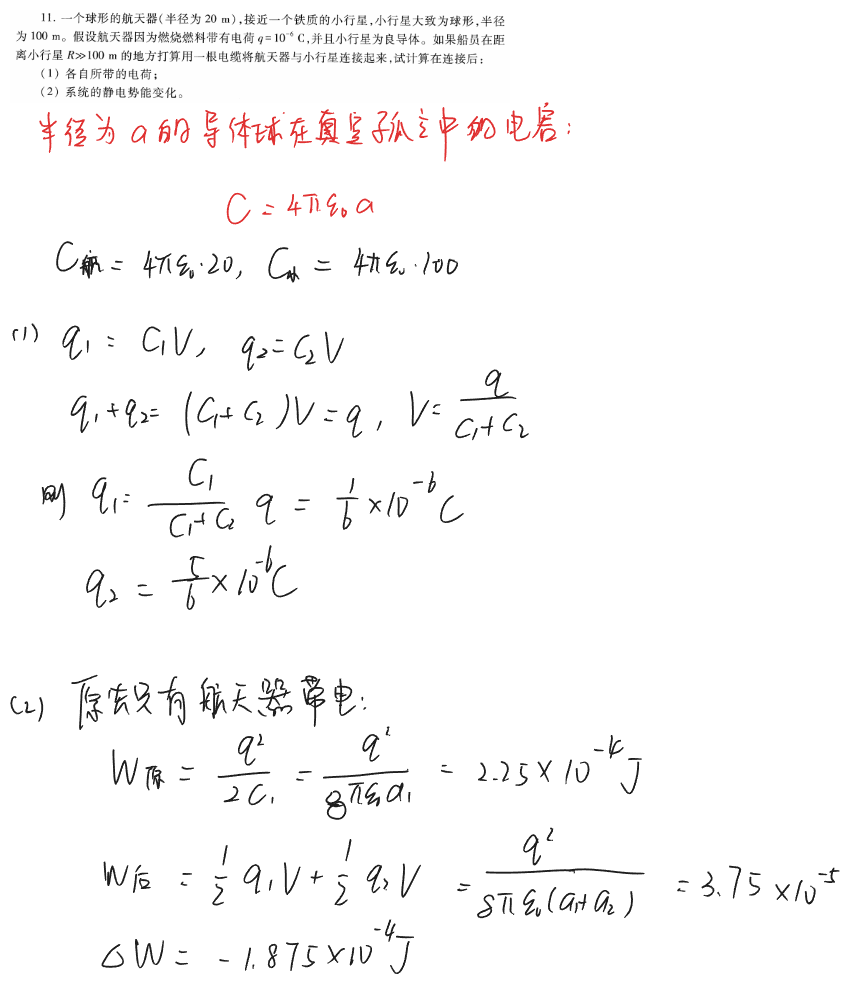
\includegraphics[width=\linewidth, height=0.88\textheight, keepaspectratio]{习题 3.1.11.png}
\end{figure}

\clearpage

% 本章习题 3.1
\section*{本章习题 1}

\begin{figure}[H]
  \centering
  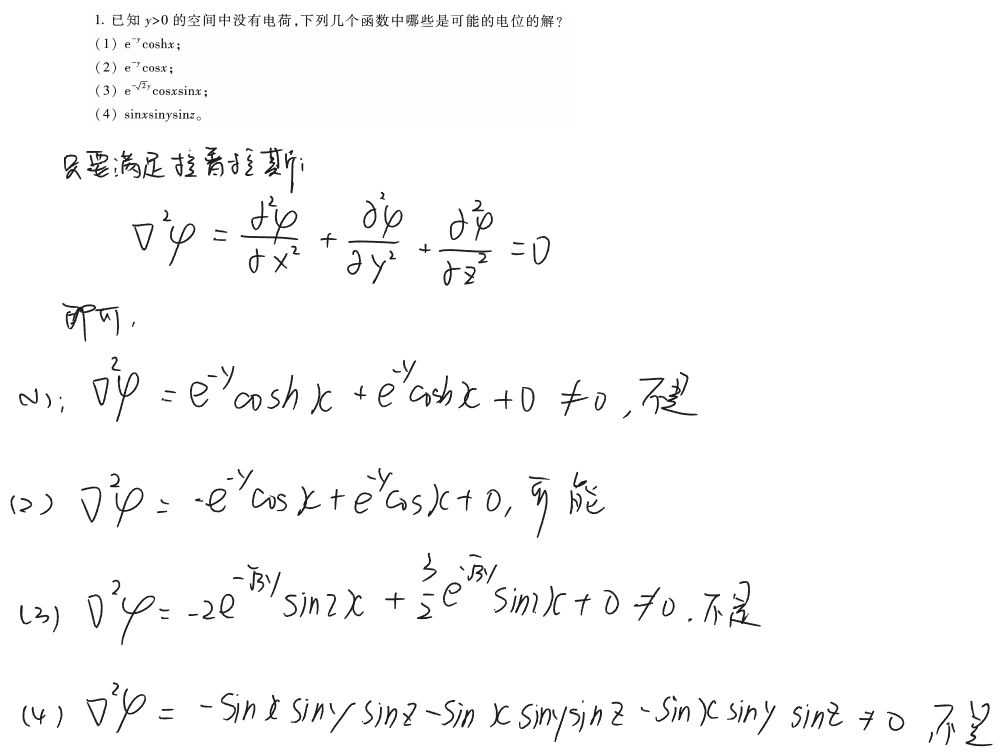
\includegraphics[width=\linewidth, height=0.88\textheight, keepaspectratio]{本章习题 3.1.png}
\end{figure}

\clearpage

% 本章习题 3.4
\section*{本章习题 4}

\begin{figure}[H]
  \centering
  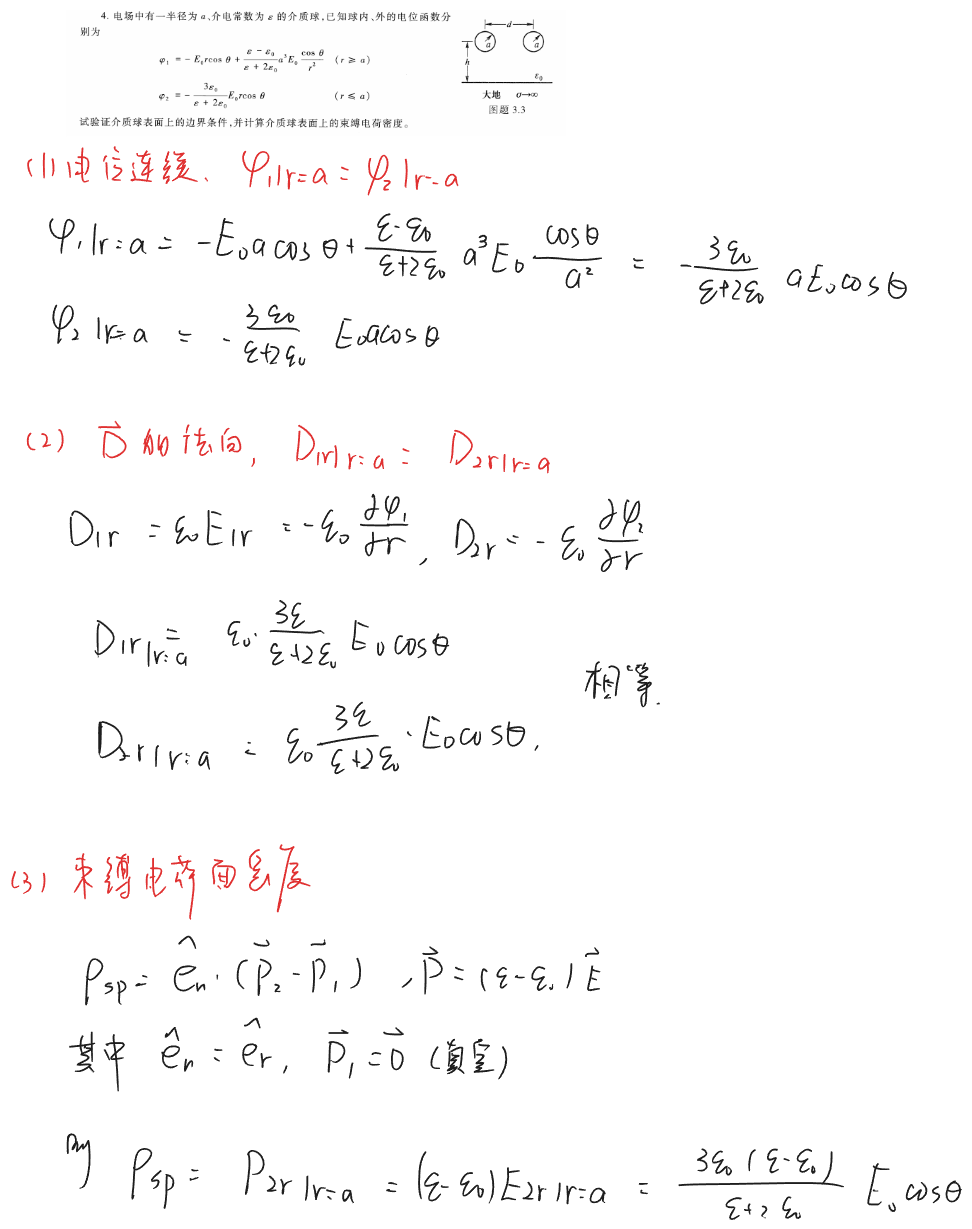
\includegraphics[width=\linewidth, height=0.88\textheight, keepaspectratio]{本章习题 3.4.png}
\end{figure}

\clearpage

% 本章习题 3.6
\section*{本章习题 6}

\begin{figure}[H]
  \centering
  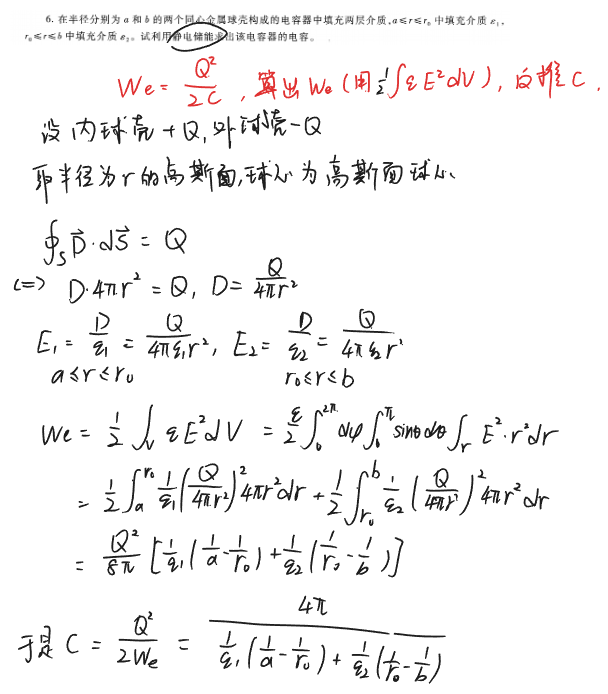
\includegraphics[width=\linewidth, height=0.88\textheight, keepaspectratio]{本章习题 3.6.png}
\end{figure}

\end{document}
